\chapter{Automation}\label{chapter:Automation}
In the last chapter, we formulated incidence claims in terms of point-sets, characterised by Theorems~\ref{rule:colltwo}--\ref{rule:collcollplane} from Figure~\ref{fig:PointSets}. These allowed us to write much shorter verifications~\cite{ScottMScThesis} than had been obtained by Meikle and Fleuriot~\cite{MeikleFleuriotFormalizingHilbert}, just using the theorem prover's stock automation. But we knew we could do better. The patterns that appeared in these verifications, which we shall refer to as our \emph{manual} verifications, were ripe for additional automation.

The HOL~Light proof assistant expects its users to work ``close to the metal'', writing ML directly. In this environment, users become comfortable prototyping and  integrating new tools. In this chapter, we shall describe the integration of an automated tool for incidence reasoning, which can be made available as a procedural tactic and to Mizar~Light proof steps.

Much of this chapter and the subsequent chapter is an expansion and improvement on earlier work~\cite{ScottExploring,ScottComposable,ScottCombinator}. In it, we shall show how the user and tool can assist each other concurrently, thereby collaborating as the user develops a proof.

\section{Background}
So far as fully automated theorem proving goes, the oldest successes are probably in geometry. Unfortunately, the approaches used assume much more than the very general theory of incidence that we consider here, and so we have had to develop our own methods. We just briefly mention some others.

\subsection{Wu's Method}
When considering general automation in Hilbert's \emph{Grundlagen der Geometrie}, there is probably no work more relevant than Wu's method~\cite{WuMechanicalTheoremProving}. Wu credited the \emph{Grundlagen} for the metatheoretical insights that led to his mechanisation procedure for the whole of geometry.

One of those insights was that the method of proof in a synthetic geometry system such as Hilbert's often falls short of absolute rigour because degenerate cases are routinely missed. Typically, when we state axioms and properties of some geometric figure, we have in mind a ``genericity'' of that figure which is hard to capture formally. Moreover, our statements may admit some generalisation to what we would regard as degenerate cases, even if this is not immediately clear at the time. We have already seen that some of Hilbert's axioms, such as Axiom~\ref{eq:g11}, when combined with other axioms, generalise to degenerate cases, and we shall see this again with Axiom~\ref{eq:g24}, which we shall strengthen in Chapter~\ref{chapter:HalfPlanes}.

But it is not always clear how the conditions in our statements can be relaxed. Moreover, when trying to rule out certain degenerate cases, there are plenty that are easily missed. When we formalise, we cannot simply neglect them unless we have proof tools that can do it for us. Filling in all the gaps requires enormous effort and complication of the verification, so it would seem that Wu is correct: we cannot be truly rigorous unless we can systematically deal with degenerate conditions. This provides an alternative way to diagnose the gaps in Hilbert's proofs spotted by Meikle and Fleuriot~~\cite{MeikleFleuriotFormalizingHilbert}: they were gaps concerning degeneracy conditions about point incidence.

Wu's highly celebrated method automatically inserts non-degeneracy conditions as it carries out proofs, and if possible, it automatically deletes redundant conditions to keep results generic. The method has been used to automatically prove an enormous number of non-trivial results in unordered geometry \cite{MechanicalGeometryTheoremProving}.

For ordered geometry, Wu extended his method by appealing to the embedding of Euclidean geometry in real-closed fields, and then applied Tarksi's well-known decision procedure. Unfortunately, the procedure is grossly intractable ~\cite{TarksiMcNaugtonReview}. Thus, in the domain of ordered geometry, which is our principle concern, Wu's Method will not be effective.

Moreover, to exploit Wu's method, we would need to show how each of his mechanical steps can be reduced to the axioms of Hilbert's system. But this reduction will presuppose some of the very elementary results which we are trying to mechanise. Indeed, Wu's method rests at least on Desargues' Theorem, which appears late on as THEOREM~53 (page 72 of the \emph{Foundations of Geometry}).

\subsection{Other Methods}
Wu's technique is algebraic, and reduces geometrical problems to polynomial equations. A similar successful method was developed as \emph{Gr\"{o}bner bases}~\cite{BuchbergerGrobner}. Like Wu's, this method automatically infers non-degeneracy conditions (though will not automatically delete redundant ones). The two techniques are comparable in the results they obtain, but in some cases, a problem soluble by one method may only be soluble by the other after some additional factorisation of the polynomial equations.

Another collection of successful methods which combine algebraic and synthetic reasoning can be described as \emph{coordinate-free} techniques~\cite{MachineProofsInGeometry}. With these techniques, it is possible to eliminate many of the non-degeneracy conditions by using generic analogues of standard geometric properties. For instance, in the area method, we generalise the notion of the area of a polygon to a \emph{signed} area according to its orientation, and in the full-angle method, we generalise the notion of an angle to an arbitrary pair of lines. Using a simple set of algebraic laws on signed areas and full-angles, it is possible to prove many geometric results \emph{and} to preserve the geometric intuition behind them. The polynomial approaches, by contrast, will produce very dense systems of equations involving dozens of variables at which point the geometric intuition is lost. 

The area method has been formalised as a Coq tactic by Narboux \cite{NarbouxAreaMethod}, while the full-angle method was used for Wilson and Fleuriot's diagrammatic geometry proof assistant \cite{GeometryExplorer}.

\section{Basis for an Algorithm}
Our own approach is based on Theorems~\ref{rule:colltwo}--\ref{rule:collcollplane}, which tell us how to reason with finite collinear and planar sets, and so can form the basis of a combinatorial algorithm. The domain of our algorithm is data representing assertions, hereafter just \emph{data}.\footnote{In our implementation, the data were precisely the sequents whose right hand side formalised the assertion, making our implementation \emph{fully expansive}~\cite{FullyExpansive}, but we could have used other data, such as a collection of proof hints, which could later be automatically processed into sequents.} There are five kinds of data: assertions that two points are equal, that two points are distinct, that a set of points is collinear, that a triple is non-collinear, and that a set of points is planar. The algorithm consists chiefly of rules and methods to generate data from other data.

These rules are similar in spirit to those given by Magaud et al~\cite{RankDesargues}. Their rules are also based on point-sets, but the authors have beautifully abstracted the core idea. In their paper, an $n$-dimensional set is assigned a \emph{rank} of $n+1$. There are then key rules which assert that, given point sets $X$ and $Y$, the sum of the ranks of $X \cup Y$ and $X \cap Y$ is no greater than the sum of the ranks of $X$ and $Y$. This abstractly characterises Theorems~\ref{rule:collunion} and~\ref{rule:planeunion} which introduce the union of collinear and planar sets respectively, while the hierarchy of ranks give us Theorems~\ref{rule:collsubset} and~\ref{rule:planesubset} for free. The use of ranks therefore identifies an analogy between how collinearity and planarity are used in our theorems.

The approach taken by Magaud et al allows them to generalise to arbitrary dimension, and the elegance of the theory helps us see our own approach as less \emph{ad hoc} than it might otherwise. For the rest of this chapter, however, we shall focus on our original, more concrete representation.

\subsection{Inference Rules}\label{list:Procedures}
Theorems~\ref{rule:colltwo}--\ref{rule:collcollplane} already show how to introduce collinear and planar sets. Additionally, we need ways to derive the inequalities and triangles which are conditions of the theorems. Firstly, we note that any triangle or non-collinear triple implies the mutual distinctness of its three points, giving us one way to introduce point inequalities. Another way to derive inequalities is through the following simple argument: suppose we have a collinear set $S$, and a non-collinear triple sharing two points with $S$. Then the third point of the triple must be distinct from all points in $S$. 

Next, we need to introduce non-collinear triples. We based our method here directly on a common pattern of reasoning from our manual verifications. Suppose we have a collinear set $S$ and a non-collinear triple sharing two points with $S$. Then the third point forms a non-collinear triple with all pairs of points in $S$ known to be distinct.

Finally, we consider how we might infer when two points are equal using our theorems. Given two collinear sets $S$ and $T$, which have a non-collinear union, we can infer that their intersection must be empty or a singleton. So if the intersection is a set of points $\{P_1,P_2,\ldots,P_n\}$, then we know immediately that these points are identical. This, we noted in the last chapter, is just telling us that distinct lines intersect in at most one point, as per Hilbert's THEOREM~1.

We now summarise the rules for introducing our five kinds of data. The first four rules apply Theorems~\ref{rule:colltwo}--\ref{rule:collcollplane} indirectly. The last five are direct.
\begin{description}
\item[$\code{ncolneq}$] Infer inequalities from non-collinear triples:
\begin{displaymath}
\vdash\neg\code{collinear}\ \{A,B,C\} \implies A \neq B \wedge A \neq C \wedge B \neq C
\end{displaymath} (by Theorem~\ref{rule:colltwo}).
\item[$\code{colncolneq}$] Infer inequalities from a collinear set containing two points of a non-collinear triple:
\begin{align*}
  &\vdash\code{collinear}\ S \wedge \neg\code{collinear}\ \{A,B,C\}\\
  &\qquad\wedge A,B \in S \implies \forall X.\;X \in S \implies C \neq X
\end{align*}(by Theorem~\ref{rule:collsubset}). For example, 
\begin{align*}
\code{collinear} \{A, B, C, D, E\} \wedge & \neg\code{collinear} \{A, B, P\}\\
&\implies A \neq P \wedge B \neq P \wedge C \neq P \wedge D \neq P \wedge E \neq P.
\end{align*}
\item[$\code{coleq}$]\label{rule:coleq}
Equate points in the intersection of two collinear sets which are jointly non-collinear:
\begin{align*}
&\vdash\code{collinear}\ S \wedge \code{collinear}\ T \wedge \neg\code{collinear}\ U \wedge U \subseteq S \cup T \\
&\qquad\qquad\wedge A,B \in S,T \implies A = B
\end{align*} (by Theorems~\ref{rule:collsubset} and \ref{rule:collunion}). For example,
\begin{align*}\
&\code{collinear} \{A, B, C, D, E\} \,\wedge\,\code{collinear} \{A, C, E, X, Y\}\\ 
&\qquad\, \wedge\,\neg\code{collinear} \{A, B, Y\}\implies A = C \wedge A = E \wedge C = E.
\end{align*}
\item[$\code{colncolncol}$] Infer new non-collinear triples from a collinear set and another non-collinear triple:
\begin{align*}
  &\vdash\code{collinear}\ S \wedge \neg\code{collinear}\ \{A,B,C\}\\
  &\qquad\wedge X,Y,A,B \in S \wedge X \neq Y\implies \neg\code{collinear}\ \{C,X,Y\}
\end{align*} (by Theorems~\ref{rule:collsubset} and~\ref{rule:collunion}). For example,
\begin{align*}
A \neq C \wedge D \neq E &\wedge \code{collinear} \{A, B, C, D, E\} \wedge \neg\code{collinear} \{A, B, P\}\\
&\implies \neg\code{collinear} \{A, C, P\} \wedge \neg\code{collinear} \{D, E, P\}.
\end{align*}
\item[$\code{colcol}$] Use Theorem~\ref{rule:collunion} to show that the union of collinear sets which intersect at more than one point is collinear.
\item[$\code{planeplane}$] Use Theorem~\ref{rule:planeunion} to show that the union of planar sets intersecting at a non-collinear triple is planar.
\item[$\code{colplane}$] Use Theorem~\ref{rule:collplane} to show that a collinear set is planar.
\item[$\code{colplaneplane}$] Use Theorem~\ref{rule:collplaneplane} to show that the union of a collinear and planar set intersecting in at least two points is planar.
\item[$\code{colcolplane}$] Use Theorem~\ref{rule:collcollplane} to show that the union of intersecting collinear sets is planar.
\end{description}

\section{Forward Chaining}\label{sec:ForwardChaining}
Forward-chaining algorithms have had recent success in automatically producing readable elementary proofs from Hilbert's axioms~\cite{ForwardChainHilbert}, and seemed particularly suitable for our use case. For instance, we found that when writing our manual verifications, we ended up with suboptimal proofs and found that the complexities of incidence reasoning left us with the suspicion that there might be errors in the prose where Hilbert had incorrectly assumed non-degeneracy conditions. We wanted a tool which could investigate these matters by exploring the proof space of incidence reasoning surrounding each of Hilbert's proofs. 

The idea of using forward-chaining in this sort of exploratory way also opened up the possibility of designing an automated tool which could collaborate with the user as they develop a verification. Forward-chaining seemed quite apt, since its focus on cumulatively growing consequences of a set of assumptions corresponds well with how a declarative verification specifies a continually growing proof context. 

Our basic approach is to produce cumulative \emph{generations} of data by combining data from previous generations. For incidence reasoning, we shall be combining the data based on the procedures of \S\ref{list:Procedures}, in the manner of forward-chaining.

\subsection{Concurrency}\label{sec:NaiveConcurrency}
Typically, the automation available in interactive proof assistants is invoked on demand by the user when they evaluate individual proof steps. But when the user writes the formal proof for the first time, or comes to edit it later, they will spend most of their time thinking, consulting texts, backtracking and typing in individual proof commands. The CPU is mostly idling during this process, and we can exploit this idle time to run automated tools concurrently.

The Isabelle proof assistant has capitalised on this with Sledgehammer~\cite{IsabelleSledgehammer}. By invoking this command, the user can continue to work on a proof, while generic first-order tools are fired off as separate background processes, attempting to solve or refute the user's goals independently. If the tools reach a conclusion, the generated proof certificates can be automatically and seamlessly integrated into the user's proof-script. 

We argue that we can do one better. We will show in~\S\ref{sec:Concurrency} how to make a forward-chaining algorithm part of a ``collaborative'' architecture. As we remarked, both declarative proof and forward-chaining share the property of growing a proof context cumulatively, so why not splice the two? The user still manually crafts a search through the proof space, but they now have access to data from a forward-chaining algorithm. At the same time, the forward-chaining algorithm works independently, but can freely incorporate the user's intermediate hypotheses as they appear in the proof context, using them for its own derivations. The two systems, the automation and the human user, can thus be seen as collaborating, sharing data as they both strive towards the goal.

%% The basic idea is very simple: we spawn a thread that is initialised with an empty generation of data. New generations are produced cumulatively through forward-chaining. At the same time, the thread monitors the proof context, so that each time the user adds a hypothesis by performing a declarative proof step, the hypothesis can be automatically inserted into the current generation and used for further chaining.

%% For the user's inspection, the thread echoes each generation of data concurrently to a separate terminal while they craft the verification. To enable the user to access the data, we introduce a variable $\code{the\_facts}$ which is updated so that when dereferenced in a verification, the current step will be justified using the latest data from forward-chaining.

%When a fixpoint is detected, the user is notified, so that they can decide whether perhaps an assumption is missing, or whether a more sophisticated subproof is needed. In the meantime, the forward-chaining thread will sleep.

%Since we are using an LCF style prover~\cite{LCF}, we always ensure that our forward-chaining derivations are fully-expansive~\cite{FullyExpansive}. This means that to carry out its derivations, the tool directly applies inference rules to generate fully machine verified lemmas. These lemmas can then be seamlessly integrated into the user's proof script to produce a fully machine-checked proof.

\subsection{Discovery}
In our designs, our automation is very much intended in the spirit of \emph{assistance}. It is not intended to take over, or to solve the user's problems. It is there as a support, to be relied on as desired. Its purposes are thus quite modest, and it may not be clear why such a tool would be so desirable. Perhaps it would be useful to set the scene.

We would typically develop our geometric proofs on paper, figuring out how to discharge non-degeneracy assumptions without any computer assistance. In our case, these assumptions required that certain points be non-equal and others non-collinear. Discharging these assumptions typically meant a pen-and-paper combinatorial search.

In this narrow domain, it was easy to imagine simple programs which could do the combinatorial search for us, and which could display a breadth of derivations in case we had missed shorter paths, or overlaps with later inferences. This, then, is not quite automated search, but more assisted search. We have chosen to give it the shorter title of \emph{discovery}, which stresses the point that we are usually interested in obtaining many derivations from the search process, including derivations we had not expected. It also stresses the point that we often did not run the searches with a concrete goal in mind. However, we should mention that our use of the word \emph{discovery} is to be contrasted with fully automated discovery systems which search for arbitrary interesting results and concepts without the need for assistance~(see the work of Colton et al.~\cite{ColtonInterestingness,MathematicalDiscovery}, McCasland and Bundy~\cite{Mathsaid}, Johansson et al~\cite{ConjectureSynthesis} and Montano-Rivas et al~\cite{SchemeBasedSynthesis,SchemeBasedConceptInvention}).

\section{An Implementation in Combinators}\label{sec:DiscoveryAlgebra}
Our domain of incidence reasoning is naturally partitioned into data of five kinds. We aimed for an implementation which respected this partitioning, thereby greatly reducing the number of combinations of data we need to try with each rule from \S\ref{list:Procedures}. These rules become the plumbing connecting the data. The data-flow model implied is given in Figure~\ref{fig:DataFlow}.

\begin{figure}
\centering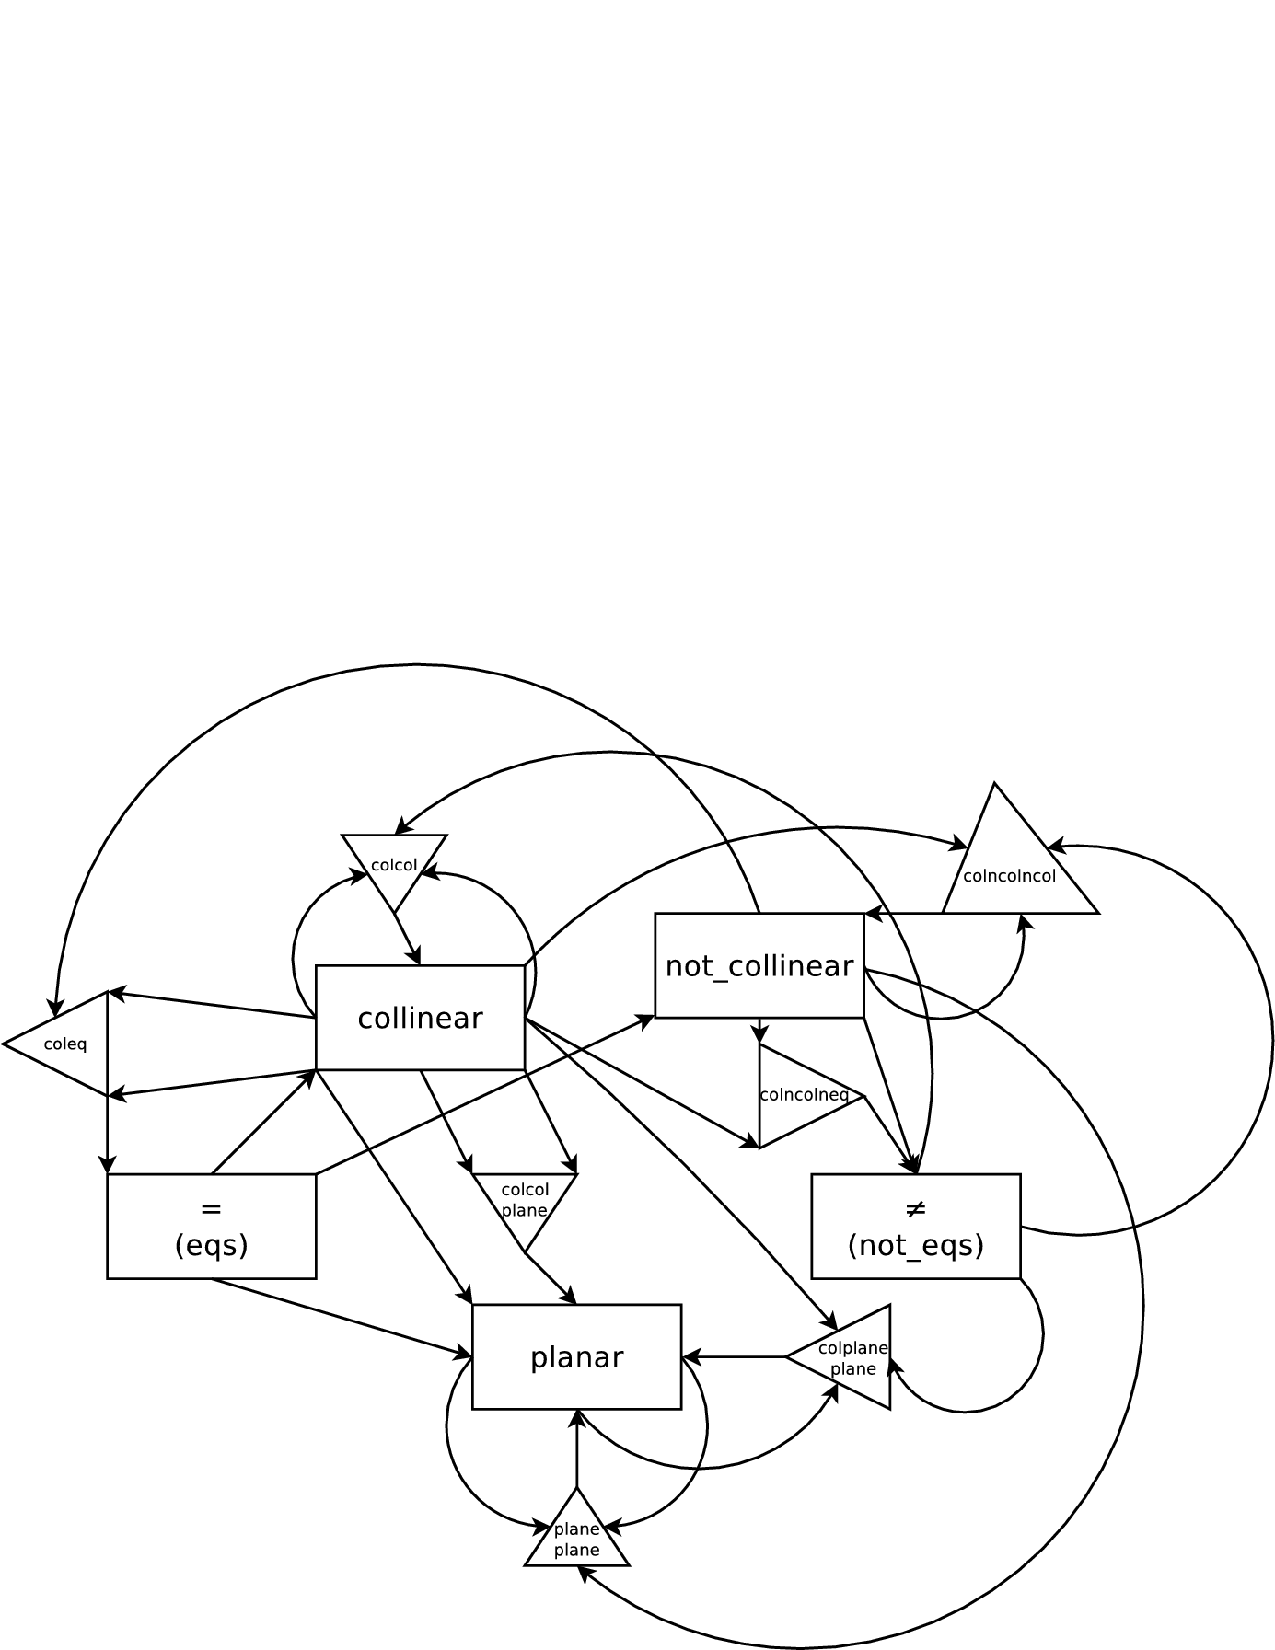
\includegraphics[scale=0.5]{automation/DataFlow}
\caption{Data-flow for incidence reasoning. The five boxes represent our five lists of data, while triangles represent inference rules}
\label{fig:DataFlow}
\end{figure}

Our aim in this section will be to show how such data-flows can be expressed declaratively in a suitable combinator language. Combinator languages are a staple of typed functional programming and LCF theorem provers, which already boast powerful combinators for conversions and tactics~\cite{Tactics}. By following the example of such languages, we hope to contribute a library that has a potentially wider application than the peculiar incidence automation we need for our verifications. The incidence automation will be just one possible hand-crafted \emph{discoverer} written in this language, just as hand-crafted tactics are written in tactic languages.

The advantage of choosing a combinator language, as opposed to some other kind of domain-specific language, is that it fully integrates with the host programming language, and is therefore easy to integrate with the tactic combinator language and the Mizar~Light combinator language. The user is also free to extend the language by defining derived combinators, and can easily inject their own computations into the language using lambda abstraction.

\subsection{Related Work}
The idea of an algebraic data-flow language was considered early on by Chen~\cite{ChenForwardChaining}, who gave a specification for a variety of primitives very similar to our own, though without an implementation. Since then, algebras for logic programming, handling unbounded and fair search have been developed~\cite{BacktrackingMonad,Omega}, but these lack strong guarantees on the order in which elements are found, and can be unpredictable.

An equivalent version of the algebra we shall consider here was originally conceived of by Spivey~\cite{SpiveyBreadthFirst}. It has been used recently by Katayama~\cite{ImprovementsMagickHaskeller} to perform exhaustive searches of functional programs, and its theoretical underpinnings have been rigorously developed~\cite{SearchAlgebras}. Unlike the other logic programming monads, it has much stronger constraints on the order in which values are searched for. 

Our own algebra generalises Spivey's implementation somewhat by replacing his \emph{bags} with more general collections, and we take advantage of this generalisation in \S\ref{sec:Trees}. Moreover, our own realisation of this algebra offers a more ``operational'' motivation of the definitions to complement Spivey's.

\subsection{Streams}\label{sec:Streams}
Our overarching purpose is to output data, perhaps to a terminal, to a database to be used during a proof, or perhaps to another consumer for further processing. If we think of this output \emph{as} the implementation, then we are dealing with procedures which lazily generate successive elements of a list. For the purposes of the theory, we assume that the lazy lists are infinite \emph{streams}. These shall be the primitives of our data-flow algebra.

For now, we leave unspecified what computations are used to generate the primitive streams. It might be that a stream simply echoes a list of precomputed data; it might generate data based on standard input; it might generate them from some other automated tool. We shall focus instead on transformations for streams, and in how we might lift the typical symbolic manipulation used in theorem proving to the level of streams.

One reason why streams and lazy lists are a good choice here is that they generalise \emph{the} ubiquitous data-structure of ML and its dialects, and have rich interfaces to manipulate them. A second reason why they are an obvious choice is that they have long been known to satisfy a simple set of algebraic identities and thus to constitute a monad~\cite{MonadWadler}. We can interpret this monad as decorating computations with non-deterministic choice and backtracking search.

Monads themselves have become a popular and well-understood abstraction in functional programming. Formally, a monad is a type constructor $M$ and three operations 
\begin{align*}
&\code{return} : \alpha \rightarrow M\;\alpha\\
&\code{fmap} : (\alpha \rightarrow \beta) \rightarrow M\;\alpha \rightarrow M\;\beta\\
&\code{join} : M\;(M\;\alpha) \rightarrow M\;\alpha
\end{align*}
satisfying the algebraic laws given in Figure~\ref{fig:MonadLaws}.

\begin{figure}
\begin{align}
&\code{fmap}\;(\lambda x.\;x)\;m = m\notag\\
&\code{fmap}\;f \circ \code{fmap}\;g = \code{fmap}\;(f \circ g)\notag\\
&\code{fmap}\;f \circ \code{return} = \code{return}\circ f\notag\\
&\code{fmap}\;f \circ \code{join} = \code{join} \circ \code{fmap}\;(\code{fmap}\;f)\notag\\
&(\code{join} \circ \code{return})\;m = m\notag\\
&(\code{join} \circ \code{fmap}\;\code{return})\;m = m\notag\\
&\code{join} \circ \code{join} = \code{join} \circ \code{fmap}\;\code{join} \label{eq:JoinAssoc}
\end{align}
\caption{The monad laws}
\label{fig:MonadLaws}
\end{figure}

The monad that is typically defined on lists can be used for search, but it takes concatenation $\code{concat} : [[\alpha]] \rightarrow [\alpha]$ for its \code{join} operation. This makes it unsuitable for \emph{fair} and \emph{unbounded search} with infinite streams. If the stream $xs$ represents one unbounded search, then we have $xs + ys = xs$ for any $ys$, and thus, all items found by $ys$ are lost.\footnote{Here, $+$ is just list and stream append.} This is to be expected, since the definition of this standard monad corresponds to \emph{depth-first search}. 

\subsection{A Monad for Breadth-First Search}\label{sec:StreamMonad}
There is an alternative definition of the monad which is breadth-first and thus handles unbounded search. Here, the \code{join} function takes an infinite stream of infinite streams, and produces an exhaustive enumeration of all elements. We show how to achieve this in Figure~\ref{fig:ShiftGen} using a function $\code{shift}$, which moves each stream one to the ``right'' of its predecessor. We can then exhaustively enumerate every element, by enumerating each column, one-by-one, from left-to-right. 

\begin{figure}
  \small
  \centering
  \begin{tabular}{rl}
    shift &
    \begin{tabular}{ccccccc}
      $[[D_{0,0},$ & $D_{0,1},$ & $D_{0,2},$ & $\ldots,$ & $D_{0,n},$ & $\ldots],$ \\
      $[[D_{1,0},$ & $D_{1,1},$ & $D_{1,2},$ & $\ldots,$ & $D_{1,n},$ & $\ldots],$ \\
      $[[D_{2,0},$ & $D_{2,1},$ & $D_{2,2},$ & $\ldots,$ & $D_{2,n},$ & $\ldots],$ \\
      $[[D_{3,0},$ & $D_{3,1},$ & $D_{3,2},$ & $\ldots,$ & $D_{3,n},$ & $\ldots],$ \\
      $[[D_{4,0},$ & $D_{4,1},$ & $D_{4,2},$ & $\ldots,$ & $D_{4,n},$ & $\ldots],$ \\
      $[[D_{5,0},$ & $D_{5,1},$ & $D_{5,2},$ & $\ldots,$ & $D_{5,n},$ & $\ldots],$ \\
      & & & & & \vdots
    \end{tabular}\\\\
    = &
    \begin{tabular}{ccccccccccccc}
      $[[D_{0,0},$ & $D_{0,1},$ & $D_{0,2},$ & $D_{0,3},$ & $D_{0,4},$ & $D_{0,5},$ & $D_{0,6},$ & \colorbox{gray}{$D_{0,7},$} & $D_{0,8},$ & $\ldots],$\\
      & $[D_{1,0},$ & $D_{1,1},$ & $D_{1,2},$ & $D_{1,3},$ & $D_{1,4},$ & $D_{1,5},$ & \colorbox{gray}{$D_{1,6},$} & $D_{1,7},$ &  $\ldots],$\\
      && $[D_{2,0},$ & $D_{2,1},$ & $D_{2,2},$ & $D_{2,3},$ & $D_{2,4},$ & \colorbox{gray}{$D_{2,5},$} & $D_{2,6},$ & $\ldots],$\\
      &&& $[D_{3,0},$ & $D_{3,1},$ & $D_{3,2},$ & $D_{3,3},$ & \colorbox{gray}{$D_{3,4},$} & $D_{3,5},$ & $\ldots],$\\
      &&&& $[D_{4,0},$ & $D_{4,1},$ & $D_{4,2},$ & \colorbox{gray}{$D_{4,3},$} & $D_{4,4},$ & $\ldots],$\\
      &&&&& $[D_{5,0},$ & $D_{5,1},$ & \colorbox{gray}{$D_{5,2},$} & $D_{5,3},$ & $\ldots],$\\
      &&&&&& $[D_{6,0},$ & \colorbox{gray}{$D_{6,1},$} & $D_{6,2},$ & $\ldots]$\\
      &&&&&&&         &        & $\vdots$ &           &        &           
    \end{tabular}
  \end{tabular}
  \caption{Shifting}
  \label{fig:ShiftGen}
\end{figure}

If we understand these streams as the outputs of a discoverer, then the outer stream can be understood as the output of a discoverer which \emph{discovers discoverers}. The \code{join} function can then be interpreted as \emph{forking} each discoverer at the point of its creation and combining the data into the output of a single discoverer. The highlighted column in Figure~\ref{fig:ShiftGen} is this combined result: a set of values generated simultaneously and thus having no specified order (this is required to satisfy Law~\ref{eq:JoinAssoc} in Figure~\ref{fig:MonadLaws}).

However, this complicates our stream type, since we now need additional inner structure to store the combined values. We will refer to each instance of this inner structure as a \emph{generation}, following our terminology from \S\ref{sec:ForwardChaining}. Each generation here is a finite collection of simultaneous values discovered at the same level in a breadth-first search. We just need to define the \code{join} function, taking care of this additional structure.

Suppose that generations have type $G\;\alpha$ where $\alpha$ is the element type. The manner in which we will define our \code{shift} and \code{join} functions on streams of generations assumes certain algebraic laws on the generations: firstly, they must constitute a monad; secondly, they must support a sum operation \mbox{$(+):G\;\alpha\rightarrow G\;\alpha\rightarrow G\;\alpha$} with identity~$0:G\;\alpha$. 

The \code{join} function for streams must then have type $[G\;[G\;\alpha]] \rightarrow [G\;\alpha]$, sending a stream of generations of streams into a stream of generations of their data. To define it, we denote the $k^{\text{th}}$ element of the argument to \code{join} by $gs_k = \{d_{k,0}, d_{k,1}, \ldots, d_{k,n}\}$ of type $G\;[G\;\alpha]$. Each $d_{k,i}$ is, in turn, a stream $[g^k_{i,0}, g^k_{i,1}, g^k_{i,2}, \ldots] : [G\;\alpha]$. We invert the structure of $gs_k$ using a function $\code{transpose}  : M[\alpha]\rightarrow [M\;\alpha]$. This function generalises matrix transposition on square arrays (type $[[\alpha]]\rightarrow[[\alpha]]$) to arbitrary monads $M$, and the generality allows us to abstract away from Spivey's bags and consider more exotic inner data-structures.\footnote{The operator \code{::} is \emph{cons} for lists and streams.}
\begin{displaymath}
\code{transpose}\;xs = \cons{\code{fmap}\;\code{head}\;xs}{\code{transpose}\; (\code{fmap}\;\code{tail}\;xs)}.
\end{displaymath}

The transpose produces a stream of generations of generations (type $[G\;(G\;\alpha)]$). If we join each of the elements, we will have a stream $[D_{k,0}, D_{k,1}, D_{k,2}, \ldots] : [G\;\alpha]$ (see Figure~\ref{fig:Transpose}), and thus, the shift function of Figure~\ref{fig:ShiftGen} will make sense. Each row is shifted relative to its predecessor by prepending the 0 generation, and the columns are combined by taking their sum.

\begin{figure}
  \begin{align*}
    &\code{map}\;\code{join}\;(\code{transpose}\;\{d_{k,0}, d_{k,1}, \ldots, d_{k,n}\})\\
  = &\code{map}\;\code{join}\;\left(\code{transpose}\;\left\{\begin{matrix}
        [g^k_{0,0}, & \colorbox{gray}{$g^k_{0,1}$}, & g^k_{0,2}, &\ldots]\\
        [g^k_{1,0}, & \colorbox{gray}{$g^k_{1,1}$}, & g^k_{1,2}, &\ldots]\\
                  & \vdots\\
        [g^k_{n,0}, & \colorbox{gray}{$g^k_{n,1}$}, & g^k_{n,2}, &\ldots]
      \end{matrix}\right\}\right)\\
      = &\left[\begin{matrix}
        \code{join}&\{g^k_{0,0}, & g^k_{1,0}, &\ldots, & g^k_{n,1}\},\\
        \code{join}&\Big\{\colorbox{gray}{$g^k_{0,1}$}, & \colorbox{gray}{$g^k_{1,1}$}, &\colorbox{gray}{$\ldots$}, & \colorbox{gray}{$g^k_{n,1}$}\Big\},\\
        \code{join}&\{g^k_{0,2}, & g^k_{1,2}, &\ldots, & g^k_{n,2}\},\\
                   & \vdots
                 \end{matrix}\right]\\
      \quad= &[D_{k,0}, D_{k,1}, D_{k,2}, \ldots]
  \end{align*}
\caption{\code{transpose} and \code{join}}
\label{fig:Transpose}
\end{figure}

The type of streams now constitutes a monad (see Spivey~\cite{SearchAlgebras} for details). The fact that we have a monad affords us a tight integration with the host language in the following sense: we can lift arbitrary functions in the host language to functions on streams, and combine one stream $xs : [G\;\alpha]$ with another stream $xs' : \alpha \rightarrow [G\;\beta]$ which depends, via arbitrary computations, on each individual element of $xs$. 

There is further algebraic structure in the form of a monoid:\footnote{A structure with an associative operation and identity.} streams can be summed by summing corresponding generations, an operation whose identity is the infinite stream of empty generations. 

\section{Case-analysis}\label{sec:CaseAnalysis}
Our algebra allows us to partition our domain into discoverer streams according to our own insight into a problem, and compose them in a way that reflects the typical reasoning patterns found in the domain. For incidence reasoning, we divide the domain into our five kinds of data discoverer, and combine the discoverers using our rules.

We wanted more than this, however, because when it comes to theorem-proving, the data is further partitioned as we perform case-analyses on disjunctions. In proof-search, when we encounter a disjunction, we will want to branch the search and associate data in each branch with its own disjunctive hypothesis. 

Ideally, we want to leave such case-splitting as a book-keeping issue in our algebra, and so integrate it into the composition algorithm. Streams must then record a context for all of their data, and this context must be respected as the streams are combined. 

Our definitions give us the flexibility to implement this. We can choose a data-structure other than bags for the generations, and to solve the problem of case-analysis, we have chosen to implement the generations as \emph{trees}. 

\subsection{Trees}\label{sec:Trees}
Each tree represents a generation of data partitioned according to case-splits. Each node in a tree is a bag of data discovered in that generation under a disjunctive hypothesis. Branches correspond to case-splits, with each branch labelled for the disjunct on which case-splitting was performed. The branch labels along any root-path therefore provide a context of disjunctive hypotheses for that subtree. For example, the tree in Figure~\ref{fig:BasicTreeExample} might represent formula~\ref{eq:CaseAnalysisTreeFormula}, made by case-analysing \mbox{$P \vee (Q \wedge (R \vee S))$}. Our goal is to discover data which hold when the case-splits are eliminated.

\begin{equation}\label{eq:CaseAnalysisTreeFormula}
\begin{aligned}
\phi_1 \wedge \phi_2 \wedge \cdots \wedge \phi_n &\wedge (P \implies \psi_1 \wedge \psi_2 \wedge \cdots \wedge \psi_n)\\
&\wedge \left(\begin{aligned} Q \implies \chi_1 \wedge \chi_2 \wedge \cdots \chi_n &\wedge (R \implies \alpha_1 \wedge \alpha_2 \wedge \cdots \wedge \alpha_n)\\ &\wedge (S \implies \beta_1 \wedge \beta_2 \wedge \cdots \wedge \beta_n)\end{aligned}\right).
\end{aligned}
\end{equation}

\subsubsection{Combining Trees}\label{fig:CombiningTrees}
\begin{figure}
\centering\includegraphics[scale=0.7]{automation/BasicTreeExample}
\caption{A simple tree branching on case-splits}
\label{fig:BasicTreeExample}
\end{figure}

The principal operation on trees is a sum function which is analogous to the append function for lists and streams, combining all data from two trees. The simplest way to combine two trees, one which yields a monad, has us nest one tree in the other. That is, we replace the leaf nodes of one tree with copies of the other tree, and then flatten. For definiteness, and to ensure associativity, we always nest the right tree in the left. See Figure~\ref{fig:TreeNesting}.

\begin{figure}
\centering\includegraphics[scale=0.7]{automation/FullSimpTree1}
\caption{Combining trees by nesting}
\label{fig:TreeNesting}
\end{figure}

Even if we only had a constant number of case-splits, successive combining in this manner would yield trees of arbitrarily large topology, which is clearly not desirable. As such, we need some way to simplify the resulting trees. Our hard constraint is that we must not lose any information: if data is deleted from the tree, it must be because it is trivially implied by other data in the tree. Our softer constraint, which we do not attempt to formally define, is that the topologies should represent a reasonably efficient partitioning of the proof-space according to the combination of case-analyses.

Our first means of simplification is a form of weakening. If we have tree $t$ which branches on a disjunctive hypothesis and which contains a subtree $t'$ branching on that same hypothesis, then the root path is of the form 
\begin{displaymath}
P \implies \cdots \implies Q \implies \cdots \implies Q \implies \phi.
\end{displaymath}
We eliminate the redundant antecedent by folding $t'$ into its immediate parent. Any siblings of $t'$ whose branch labels are not duplicated along the root path are then discarded. They will be left in the other branches of $t$.

The situation is shown in Figure~\ref{fig:TreeWeakening}, where we have coloured duplicate hypotheses along root paths. In the result, we fold the marked subtrees into their parents, and discard the siblings. Notice that no data has been lost, and no individual bags at tree-nodes have been changed: the only operations we use here are topological changes to the tree, and bag union $(+)$.

\begin{figure}
\centering\includegraphics[scale=0.6]{automation/FullSimpTree2}
\caption{Weakening}
\label{fig:TreeWeakening}
\end{figure}

Our next simplification allows us to delete a subtree $t$ if its branch case is already considered by an uncle\footnote{The sibling of a parent node.} $t'$. All theorems of $t$ will appear in $t'$ where the topology will have been simplified in our weakening step. The situation is shown in Figure~\ref{fig:TreeRedundantSplits}. The $P$ branch on the left-hand side is uncle to the $P$ branches on the right. These latter branches are therefore pruned.

\begin{figure}
\centering\includegraphics[scale=0.7]{automation/FullSimpTree3}
\caption{Removing redundant case-splits}
\label{fig:TreeRedundantSplits}
\end{figure}

Finally, we can promote data that appears at all branches. In Figure~\ref{fig:TreeRedundantSplits}, the $xs'$ bag of theorems appears in every node at the same level, and so can be promoted into the parent, corresponding to disjunction elimination. 

Our final tree is shown in Figure~\ref{fig:TreePromoting}. We have described our simplification in several steps, though they can be combined into a single pass of the left hand tree. That said, with a single pass, we have not found a way promote \emph{all} data. If we had, the replicated $us'$ bag in the bottom right branches of the tree could be promoted into the $Q$ branch. We will not elaborate on this implementation issue.

\begin{figure}
\centering\includegraphics[scale=0.7]{automation/FullSimpTree4}
\caption{Promoting common data}
\label{fig:TreePromoting}
\end{figure}

\subsubsection{Joining Trees}
Our function which combines trees is a sum function, which has an identity in the empty tree containing a single empty root node. This is enough structure to define a \code{join} function analogous to list and stream concatenation. Suppose we are given a tree $t$ whose nodes are themselves trees (so the type is $\code{Tree}\;(\code{Tree}\; \alpha)$). Denote the inner trees by $t_0$, $t_1$, $t_2$, $\ldots$, $t_n : \code{Tree}\;\alpha$. We now replace every node of $t$ with an empty bag, giving a new tree $t' : \code{Tree}\;\alpha$. We can now form the sum 
\begin{displaymath}
t' + t_0 + t_1 + t_2 + \cdots + t_n.
\end{displaymath}

The resulting tree will then contain discovered data which respect disjunctive hypotheses from their place in $t$ and from their respective inner-trees.

\section{Additional Primitives and Derived Discoverers}\label{sec:Additional}
Using trees as generations, we have a stream data-type to represent a discoverer searching a space which has been partitioned according to case-splits. Since we do not specify what sort of data we are considering, our discoverers have polymorphic type. We alias the type as $\code{discoverer}\ \alpha$. 

As we described in \S\ref{sec:StreamMonad}, these discoverers form a monoid. Operationally, the sum function runs two discoverers in parallel, respecting their mutual case-splits, while our identity discovers nothing but empty generations.

We now explain additional functionality, some of which relates specifically to theorem proving and some of which more generally handles filtering. The following material, so far as we are aware, is new.

\subsection{Case-splitting}
Case-splits are introduced by our function $\code{disjuncts}$, which is a discoverer parameterised on arbitrary sequents. Here, $\code{disjuncts}\left(\Gamma \vdash P_1 \vee P_2 \vee \cdots \vee P_n\right)$ is a stream containing a single tree with $n$ branches from the root node. The $i^{th}$ branch is labelled with the term $P_i$ and contains the single sequent $\Gamma \cup \{P_i\} \vdash P_i$. This process can be undone by flattening trees using $\code{flatten}$, which discharges all tree labels and adds them as antecedents in the right hand side of all sequents.

\subsection{Delaying}
A generation can be ``put off'' to a later generation using the function $\code{delay}$. In terms of streams, this function has the trivial definition
\begin{displaymath}
  \code{delay}\ xs = \cons{\emptyset}{xs}.
\end{displaymath}
The use of this function is actually essential when writing mutually recursive discoverers. If one discoverer outputs data based on data output by another discoverer, and \emph{vice versa}, then one of the two discoverers must be delayed to avoid deadlock.

\subsection{Filtering}\label{sec:Filtering}
In many cases, we will not be interested in all the outputs generated by a discoverer. Fortunately, filtering is a library function for monads with a zero element, and can be defined in terms of the usual bind operation ($\bind$). We give definitions for both $(\bind)$ and $\code{filter}$ as follows:
\begin{align*}
xs \bind f &= \code{join}\;(\code{fmap}\;f\;xs) \\
\code{filter}\;p\;xs &= xs \bind (\lambda x.\;\code{if } p\;x \code{ then } \code{return}\;x \code { else } 0).
\end{align*}

More challenging is a function to perform something akin to \emph{subsumption}. The idea here is that when a sequent is discovered which ``trivially'' entails a later sequent, the stronger sequent should take the place of the weaker. This is intended only to improve the performance of the system by discarding redundant search paths based on subsumed sequents. 

We can generalise the idea to arbitrary data-types, and parameterise the filtering by any partial-ordering on the data, subject to suitable constraints. One intuitive constraint is that a stronger item of data should only replace a weaker item so long as we do not ``lose'' anything from later discovery. Formally, we require that any function $f$ used as the first argument to \code{fmap} is monotonic with respect to the partial-order. That is, if $x \leq y$ then $f(x) \leq f(y)$. 

We then implement ``subsumption'' as the transformation \code{maxima}. This transforms a discoverer into one which does two things: firstly, it transforms every individual generation into one containing only maxima of the partial-order. Secondly, it discards data in generations that is strictly weaker than some item of data from an earlier generation. To handle case-splits, we assert that data higher up a case-splitting tree is always considered stronger than data below it (since it carries fewer case-splitting assumptions).

\subsubsection{More Sophisticated Filtering}
There are two pieces of missing optimisation. Suppose we have data $x$ and $y$ where $x \leq y$ and a stream $xs = \left[\{x\}, \{y\}\right].$ That is, $xs$ represents a discoverer which produces two generations of data. In the first generation is the single datum $x$ and in the second is the single datum $y$. Now suppose we have a function $f$ which happens to have the mappings
\begin{align*}
x &\mapsto \left[\{\},\{\},\{\},\{\},\{x'\}\right]\\
y &\mapsto \left[\{y'\}\right].
\end{align*}

Here, $y$ is sent immediately to the new datum $y'$, while the image $x'$ of $x$ takes some time to generate, represented here by a succession of four empty generations. Thus,
\begin{displaymath}
xs \bind f = \left[\{y'\}, \{\}, \{\}, \{\}, \{x'\}\right].
\end{displaymath}

What happens when we want to take the maxima of this stream? To do this, $f$ must be monotonic, and to verify this, we need some way to partially order the images of $f$, which means knowing more generally how to partially order discoverers.

In general, if two discoverers $xs$ and $ys$ are such that $xs \leq ys$, what should we say this implies about the ordering of the items discovered by each? We should be able to say at least this much: for every $w$ in the first $n$ generations of $xs$, there should exist some $z$ in the first $n$ generations of $ys$ such that $w \leq z$. Thus, $ys$ discovers data which is at least as strong as the data of $xs$, and does so at least as early in terms of the number of generations.

So if by monotonicity we require that $\left[\{\},\{\},\{\},\{\},\{x'\}\right] \leq \left[\{y'\},\{\}\right]$, then we further require that $x' \leq y'$. Therefore:
\begin{displaymath}
\code{maxima}\ xs \bind f = \code{maxima}\ \left(\left[\{y'\}, \{\}, \{\}, \{\}, \{x'\}\right]\right) = \left[\{y'\}, \{\}, \{\}, \{\}, \{\}\right].
\end{displaymath}
And here we have a problem: the delayed and potentially slow computation of $x'$ was wasted. Once $y$ was discovered, further discovery based on $x$ should have been halted. This does not happen in our implementation, and leads to a great deal of wasted effort. Consider the fact that every time we successfully apply Rule~\code{colcol} to take the union of sets $S$ and $T$, all further discovery based on $S$ and $T$ should be abandoned in favour of discovery using $S \cup T$. A similar issue applies to the discovery of equalities: as new equalities are discovered, they should rewrite all other data and ongoing discovery based on unwritten data should be abandoned.

A second piece of potentially desirable functionality is a form of \emph{memoisation}. Suppose two generations of a discoverer are evaluated to $[\{x\}, \{y\}]$ where $x \leq y$. With $y$ evaluated, we would probably prefer any reevaluation of this discoverer to actually replace $x$, yielding $[\{y\}, \{\}]$. 

This additional functionality has not yet been implemented, and to get it to work, we might have to significantly modify the underlying data-structures for our streams. We leave such possibilities to future work.

\subsection{Accumulating}\label{sec:Accumulating}
We supply an accumulation function which is similar to the usual \code{fold} function on lists and streams. This threads a two-argument function through the data in a stream, starting with a base-value, and folding each generation down to a single intermediate datum. Thus, we have:
\begin{align*}
\code{accum}\;(+)\;0\;[\{1,2\}, \{3,4\}, \{5\}, \{6,7,8\}] 
&= [\{0 + 3\}, \{3 + 7\}, \{10 + 5\}, \{15 + 21\}]\\
&= [\{3\}, \{10\}, \{15\}, \{36\}].
\end{align*}

One useful case of this allows us to gather up all data discovered so far in a single collection. If the collection is finite lists, we just use $\code{accum}\;(\lambda xs.\;\lambda x.\;x :: xs)\;[\,]$.

% \subsection{Normalisation}
% For efficiency, it will be useful to normalise with respect to any discovered equalities and simple rewrite rules. 

\subsection{Deduction}
Direct deduction, or \emph{modus ponens}, is the basis of forward-chaining and we provide two main ways to lift it into the type of discoverers. 

We first have to deal with \emph{exceptions}. In HOL~Light, the \emph{modus ponens} inference rule will throw an exception if its arguments are of incorrect form, so we first redefine \code{fmap} to filter thrown exceptions out of the discovery. It is generally undesirable to let exceptions propagate upwards, since this would lead to an entire discoverer being halted. 

With \code{fmap} redefined as \code{fmap'}, we can define functions $\code{fmap2}'$ and $\code{fmap3}'$ which lift two and three-argument functions up to the level of discoverers, also filtering for exceptions.
\begin{align*}
\code{fmap}'\;f\;xs &= xs \bind (\lambda x.\;\code{try}\; \code{return}\;(f\;x)  \code{ with \_ } \rightarrow 0)\;xs\\
\code{fmap2}'\;f\;xs\;ys &= \code{fmap}\;f\;xs \bind (\lambda f.\;\code{fmap}'\;f\;ys)\\
\code{fmap3}'\;f\;xs\;ys\;zs &= \code{fmap}\;f\;xs \bind (\lambda f.\;\code{fmap2}'\;f\;ys\;zs).
\end{align*}
With these, we can define the following forward-deduction functions:
\begin{align*}
\code{chain1}\;imp\;xs &= \code{fmap2}'\; \code{MATCH\_MP}\; (\code{return}\;imp)\;xs \\
\code{chain2}\;imp\;xs\;ys &= \code{fmap2}'\; \code{MATCH\_MP}\; (\code{chain1}\; imp\;xs)\;ys\\
\code{chain3}\;imp\;xs\;ys\;zs &= \code{fmap2}'\; \code{MATCH\_MP}\; (\code{chain2}\;imp\;xs\;ys)\;zs\\
\code{chain}\;imps\;xs &= imps \bind (\lambda imp.\;\code{if is\_imp } imp\\ &\code{then } \code{chain}\;(\code{fmap}\;(\code{MATCH\_MP}\;imp)\;thms)\;thms\\
&\code{else } \code{return}\; imp).
\end{align*}

The function \code{is\_imp} is a standard HOL~Light function which returns \code{true} if the right hand side of its sequent argument is an implication, while $\code{MATCH\_MP}$ is the matching \emph{modus ponens} derived inference rule
\begin{displaymath}\infer[\code{MATCH\_MP}]{\Gamma\cup\Delta \vdash Q'}{\Gamma \vdash P \implies Q&\Delta \vdash P'}
\end{displaymath}
where $P'=P[\theta]$ and $Q'=Q[\theta]$ for some substitutiton $\theta$. 

Thus, \code{chain1} takes a sequent $\Gamma \vdash P \implies Q$ and applies \emph{modus ponens} across a discoverer of antecedent sequents. The function \code{chain2} takes a sequent of the form $\Gamma \vdash P \implies Q \implies R$ and applies \emph{modus ponens} across two discoverers of antecedents. The function \code{chain3} takes a sequent of the form $\Gamma \vdash P \implies Q \implies R \implies S$ and applies \emph{modus ponens} across three discoverers of antecedents. The final, more general \code{chain} function, recursively applies implication sequents with arbitrary numbers of curried antecedents from the discoverer $imps$ across all possible combinations of antecedents from the discoverer $xs$.%, reproducing the behaviour of \sec{sec:Example}.

Note that the discoverers \code{chain1}, \code{chain2} and \code{chain3} will not necessarily try all combinations of theorems from their arguments. They fail opportunistically, attempting \emph{modus ponens} on each sequent from the first argument, and \emph{only if it succeeds}, attempting \emph{modus ponens} on sequents from the second argument. This is a happy feature of the data-driven semantics of monads (but see \S\ref{sec:Applicative} for its drawbacks). 

It is therefore sensible to order the antecedents of the implication according to how likely they are to succeed. Antecedents which rarely succeed should appear early to guarantee a quick failure. In our use case, for example, we apply Rule \code{coleq} from \S\ref{rule:coleq} with the collinear antecedents before the non-collinear antecedent, since there are generally many more non-collinear sequents to choose from than there are collinear sequents.

% CHAIN_MP, CHAIN1, CHAIN2, CHAIN3

% Not listed are functions based on Modus Ponens (\code{mp}). These functions we have called \code{chain1}, \code{chain2}, \code{chain3}, and so on, each written in one line of code in terms of its predecessor. The function \code{chain\_n} takes an implicational rule with $n$ antecedents, and yields a function which takes $n$ antecedent discoverers to produce a conclusion discoverer. 

% Our implementation allows for some interesting control of the search when discoveres are combined in this way. Antecedents in the original rule are matched one at a time, and conjunctions are split after each match. By carefully ordering and interleaving antecedents in the original rule around conjunctions, the user can control the search strategy. For example, suppose we create functions of three chains by applying 

% \noindent\code{   chain3 : thm $\rightarrow$ thm chain $\rightarrow$ thm chain $\rightarrow$ thm chain $\rightarrow$ thm chain} 

% \noindent to the equivalent rules:
% \begin{align*}
% &(P \rightarrow S \rightarrow Q \rightarrow X) \wedge (Q \rightarrow T \rightarrow P \rightarrow Y)
% \shortintertext{and}
% &P \rightarrow Q \rightarrow (S \rightarrow X \wedge T \rightarrow Y)
% \end{align*}

% The two resulting functions will differ in how they perform search on their three argument chains, in a potentially significant way. The first will simultaneously try to match $P$ and $Q$ in the first discoverer. Successful matches will respectively match $S$ and $T$, and then finally $Q$ and $P$. However, the second function will only try to match $P$. If successful, it will then match $Q$, and if that is successful, it will try to match $S$ and $T$ simultaneously. 

% The first formulation may be preferred when $P$ and $Q$ are equally likely to match and matches against $S$ and $T$ depend respectively on whether $P$ and $Q$ match. The second formulation would be preferred if $P$ is much less likely to match than $Q$ and there is no such dependence.

% This completes our overview of the discovery language. A user can now build discovery engines directly from these functions and primitives. This is very much in the spirit of HOL~Light and its LCF~\cite{LCF} foundation, where inference rules, tactic languages and rewrite engines are ordinary functions and combinator languages~\cite{Tactics}. Shallow-embedded tools can be a challenge for new users, but they offer enormous expressive power in a rich programming language, and allow different parts of the system to seamlessly integrate. 

\section{Integration}
It is straightforward to integrate our discoverers with the rest of HOL~Light's proof tools. We can, for example, lift term-rewriting to the level of discoverers simply by lifting HOL~Light's rewriting functions with \code{fmap} and its derivatives. 

To use our discoverers in declarative proofs, we introduce two Mizar~Light primitives. The first, \code{obviously}, is used to assist any step in a declarative proof via a discoverer.\footnote{The type \code{thm} is the type of HOL~Light sequents. The type \code{step} is the type of Mizar~Light steps.}
\begin{displaymath}
  \code{obviously}\;:\;(\code{discoverer}\ \code{thm}\rightarrow\code{discoverer}\ \code{thm}) \rightarrow step \rightarrow step.
\end{displaymath}

The expression $\code{obviously}\  f$ transforms a step into one which lifts the step's justifying theorems into a discoverer, applies the transformation $f$ to this discoverer, and then retrieves all discovered theorems to a certain depth. These are then used to supplement the step's justification.

By allowing $f$ to have type $\code{discoverer}\ \code{thm}\rightarrow\code{discoverer}\ \code{thm}$, we can use a discovery pipeline via function composition to justify a declarative step. For example, later in our formal development we will introduce an incidence discoverer $\code{by\_incidence}$. We also have a function $\code{split}$  which recursively breaks conjunctions and splits disjunctions across all sequents found by a given discover. Finally, we have a rule $\code{add\_triangles}$ which introduces non-collinearity sequents from sequents about points inside and outside triangles. The three functions can be pipelined in a single step by writing
\begin{displaymath}
\code{obviously}\ (\code{by\_incidence}\circ \code{add\_triangles}\circ \code{split}) \ldots.
\end{displaymath}

Next, we introduce a primitive $\code{clearly}$. This has the same type as $\code{obviously}$, but rather than collecting all discovered sequents, it searches specifically for the formula to be obtained by a Mizar~Light step (in the case of a $\code{qed}$ step, this is the goal formula). When the \code{clearly} primitive is used, it leaves the basic Mizar~Light justification tactic with a trivial proof.

\label{sec:DiscoverTac}
Finally, we have introduced a theorem-tactic \code{discover\_tac} with type
\begin{multline*}
\code{discover\_tac}\;:\;(\code{discoverer}\ \code{thm}\rightarrow\code{discoverer} \ \code{thm}) \\\rightarrow ([\code{thm}] \rightarrow \code{tactic}) \rightarrow \code{tactic}.
\end{multline*}
As with $\code{obviously}$ and $\code{clearly}$, we take a transformation of discoverers. Then when we apply $\code{discover\_tac}\ f\ tac$,  all goal hypotheses are fed to $f$. The resulting discovered sequents are then supplied to the function $tac$ (often just $\code{MESON}$).

\subsection{Concurrency}\label{sec:Concurrency}
In \S\ref{sec:NaiveConcurrency}, we hinted at the possibility of making our algorithm concurrent and collaborative. The implementation is straightforward with streams.

So that discoverers can incorporate the user's manual proof efforts, they need a way to inspect the proof context. We use a simple new primitive discoverer $\code{monitor}$ to allow this. As we stated in our introduction in \S\ref{sec:Streams}, primitive discoverers can generate their outputs in whatever manner they want. Our $\code{monitor}$ just regularly examines the proof context and outputs its hypotheses. We ensure that only unique hypotheses are ever generated by using the function $\code{maxima}$.

For the user's inspection, discovered theorems are output to the terminal one-by-one, simply by iterating over the streams with an ordinary print function in a separate thread. Additionally, this thread updates a reference cell \code{the\_facts} which holds all theorems discovered in that thread so far. The cell can be deferenced in the interactive proof, so that the user can make use of the results of concurrent discoverers as they come in.

To complete the architecture, we provide signalling commands that can tell a discovery thread to pause, thereby freeing up CPU resources, to resume from a pause, or to change to an alternative theorem discoverer, so that the thread does not have to be killed.

We should admit to a caveat here. Generations, as we have implemented them, are not generally valid across the branches of case-splits and the subproofs of a declarative verification. When the user completes a branch or subproof, some of their assumptions will no longer be in force, and further data generated from those assumptions will become unusable. Our implementation does not, as yet, address this issue. Instead, we simply reset the discoverers after each case-split and subproof.

% \begin{figure}
% {\scriptsize\input{incidence}}
% \caption{Incidence Discovery in ML}
% \label{fig:MLEngine}
% \end{figure}

\subsection{Dependency Tracking}\label{sec:WriterMonad}
While writing a proof, we would normally start our incidence discoverer concurrently, which would generate sequents as we worked. The discoverer would consider all of our goal hypotheses, and would typically find a large number of sequents, most of which were not needed in the proof. Of those which were needed, we wanted to know the specific subset of hypotheses from which they were derived. This is desirable when it comes to proof-replay, when we would like the discoverer to work more efficiently with just the hypotheses it needs. But it is also desirable in terms of writing declarative proofs: we want to write the dependent hypotheses directly into the proof script, so they are apparent to the reader. To achieve this, we need our discoverers to track hypotheses.

A nice feature of monads in functional programming is that, when defined in the form of a \emph{transformer}, the extra book-keeping can be added in a clean and modular way. In this case, we create a generic \emph{writer transformer}.

\emph{Writer} is a monad with extra functions for \emph{writing} values from any monoid during a computation, and for running computations to retrieve the final written values. It provides a modular way to introduce things such as \emph{logging} into computations. So if we have a computation which writes the value \code{"Hello"} and returns the value 1, and another computation which writes the value \code{" world!"} and returns the value 2, then when we lift addition over the two computations, we have a computation which returns the value 3 and writes \code{"Hello world!"}. The monoid here is strings with the append operation.

Writer can be defined as a transformer which, when applied, is made to write values inside any other monad. We made our writer work on a monoid of hypothesis sets with the union operation. These sets contain the dependent hypotheses from the proof context for every discovered sequent, and they automatically accumulate as discoverers are combined. We do not need to write any special logic for this. All the details are handled generically by the writer transformer.

All we need to do is extend the $\code{monitor}$ discoverer to initialise the dependent hypotheses sets. So now, every time $\code{monitor}$ pulls a hypothesis from the proof context, it must also write the hypothesis as a dependency on further computation. The dependencies then automatically propagate.

\section{Implementation Details}
The following section describes some technical challenges we faced. We include it for the sake of honesty, since the presentation of the ideas so far ignores all the bumps that thwart a nice clean implementation in Ocaml. We assume some knowledge of the Ocaml language here.

We have implemented a general monad library in Ocaml, providing a signature for the minimal implementation of an arbitrary monad, and a \emph{functor}\footnote{All uses of the term \emph{functor} here refer to a feature of the Ocaml module system. Though a term borrowed from category theory, it is not in the same context as \emph{monad} as we have used it in this chapter.} to turn this minimal implementation into a richer monad interface with derived functions. Monad transformers are functors between minimal implementations of monads. The stream monad itself is a transformer from an arbitrary monad of generations. If we want to use the bag implementation, we can just supply a module of bags to this transformer. If we want to use our case-splitting implementation, we supply our module of trees. 

These transformations can be stacked. In fact, in our final implementation, we first apply our writer transformer to a monoid of hypotheses sets. The writer transformer is then applied to our tree monad. Finally, the tree monad is applied to our stream monad to produce a stream which discovers theorems, handles case-splits and tracks dependent hypotheses.

\subsection{Implementation Issues}
As of writing, HOL~Light relies heavily on modifications to Ocaml's preprocessor, one of which forces Ocaml's lexer to treat any lexeme which contains more than one upper-case letter as being a lower-case identifier. This plays havoc with the CamelCase naming convention now being adopted in Ocaml's ``Batteries Included'' library, since Ocaml's parser expects all module names to be uppercase. To circumvent this, we supply our own preprocessor which allows for lower-case identifiers in module names. This is only intended as a hack over a hack until we find a robust solution.

Concurrency often raises thorny issues in working code, and some HOL~Light functions were not developed with concurrency in mind. The basic \code{MESON} tactic, which we rely on throughout our verifications, is not thread-safe, and it must be avoided when defining discoverers.

% We have stressed ``concurrency'' in this chapter, rather than ``parallelisation'', since Ocaml only supports the former. This means we get no speed improvements by using threads. This should not be seen as a significant drawback, since such multithreading is inherently dangerous in a language such as Ocaml which allows for uncontrolled side-effects. HOL~Light itself was not developed with multiprocessing support in mind. Its basic \code{MESON} tactic, for instance, is not thread-safe. Even without parallelisation, the tactic must be avoided when implementing discoverers.

Another issue with threading concerns UNIX signals. The standard way to interact with HOL~Light is to run intractable decision procedures on problems. If these procedures fail, the user interrupts them at the Ocaml top-level by sending \code{SIGINT}. If the user is running a concurrent discoverer when they send this signal, it might interrupt the wrong thread, possibly leaving the discoverer with dangling resources. As a quick hack around this behaviour, we trap SIGINT in the discovery thread, pause, and emit it again.

Finally, Ocaml's lazy list library has some unexpected implementation choices. For instance, the list concatenation function $concat\;:\;[[\alpha]]\rightarrow[\alpha]$ is \emph{strict} in its outer list, while the $\code{take}$ function which takes a certain sized prefix of a given lazy list will always force the values in the prefix. These behaviours are generally inappropriate for lazy data-structures, and their use often leads to infinite looping when we come to write recursive functions which generate lazy lists. We have had to rewrite many of them.

Besides these issues, the syntax for lazy lists in Ocaml is cumbersome. Primitive list functions have to explicitly force lazy lists, while recursive lazy lists must be wrapped with a \code{lazy} keyword. One benefit, however, of Ocaml's lazy list implementation is that it detects when a recursive definition requires forcing a vicious circularity. Such a scenario arises when the computation of the first element of $xs$ requires computing the first element of $ys$, and \emph{vice versa}. Such situtations occur easily when writing discoverers in our algebra, and are fixed with choice uses of the $\code{delay}$ function.

\section{Applicative Functors}\label{sec:Applicative}
An idiom or applicative functor $F$~\cite{Applicative} is a generalisation of the monad, which could be thought of as providing at least the ability to lift values with a function $pure\;:\;\alpha \rightarrow F\ \alpha$ and to lift a two argument function as we do with 
\begin{displaymath}
\code{fmap2}\;:\;(\alpha\rightarrow\beta\rightarrow\gamma)\rightarrow F\ \alpha \rightarrow F\ \beta \rightarrow F\ \gamma.
\end{displaymath}

This is actually quite limiting compared to the monad (see \cite{IdiomsArrowsMonads} for a detailed analysis). We can no longer write data-driven computations, such as our $\code{chain}$ functions which automatically fail at the first non-matching antecedent.

That said, because it does not allow data-driven computation, an implementation of the applicative functor interface can potentially be more efficient than the implementation it derives as a generalisation of a monad. This was something we spotted when fixing a performance issue with our trees.

In Figure~\ref{fig:ApplicativeSimp}, we show what happens when we lift a two argument function $f$ over two trees with the same topology. The result is correctly simplified, so that it appears that the function $f$ is evaluated exactly five times. But, bizarrely, when we came to profile our code, we found that the function $f$ was evaluated \emph{nine} times, once for each possible combination of data in the two trees. The data were discarded in simplification, but only after they were evaluated. This completely breaks the intended purpose of the trees, which is to partition the data so that the discarded computations never take place.

\begin{figure}
\centering\includegraphics[scale=0.7]{automation/BasicTreeSimp}
\caption{Applicative simplification}
\label{fig:ApplicativeSimp}
\end{figure}

The inefficiency is actually unavoidable with the monad implementation. A computation in a monad produces structure dependent on data within another structure. When we lift a two argument function over two structures, it happens that the structure of the final value is independent of this data, but the independence cannot be guaranteed by the type system.

This is the advantage of the applicative functor. In defining it, we are not allowed to peek at the data inside our structures, so when lifting a two argument function, the type system can guarantee that the final structure can only depend on the structures of the two inputs. 

For our trees in Figure~\ref{fig:ApplicativeSimp}, we know, without looking at the data, what the topology of the final result should be. We know, in advance, what simplifications should come in, and we therefore know, in advance, how many times the function $f$ will be applied. But this knowledge is only guaranteed for applicative functors. When we use the derived monad implementation, $f$ must be applied across all computations and only \emph{then}, when all dependencies on the data have been take into account,  can simplification take place.

A simple fix is to provide an explicit applicative implementation which will override the derived monad implementation. The resulting overridden interface is identical from the perspective of client code, but now, when the client does not require data driven computations, such as with the applicative functions $\code{fmap2}$, $\code{fmap3}$ and so on, the more efficient implementation is used.

\section{The Problem Revisited}\label{sec:Solution}
We now return to our original data-flow problem. In Figure~\ref{fig:IncidenceDiscoveryCode},\footnote{The inference rule \code{CONJUNCTS} sends a conjunctive sequent to a list of its conjuncts.} we use our discovery algebra to capture the complex data-flow network from Figure~\ref{fig:DataFlow}. As we can see, the five kinds of data now correspond to five primitive discoverers. Rules are applied across the data by lifting those rules into the type of discoverers, and mutual dependencies of the network are captured by mutual recursion.
\begin{figure}
\begin{align*}
&\hspace{-2.55cm}\code{sum} = \code{foldr}\ (+)\  0\circ \code{map}\ \code{return}\\
&\hspace{-2.55cm}\code{conjuncts} = \code{fmap'}\ \code{CONJUNCTS}\\\\
\code{by\_incidence}\ thms = \\
\quad \code{let rec}\ collinear =& \code{maxima}\ (\code{filter}\ \code{is\_collinear}\ thms\\
& + \code{fmap3'}\ \code{colcol}\ (\code{delay}\ collinear)\ (\code{delay}\ collinear)\\
&\qquad\qquad neqs)\\
\code{and}\ non\_collinear =& \code{maxima}\ (\code{filter}\ \code{is\_non\_collinear}\ thms\\
&+ \code{fmap3'}\ \code{colncolncol}\ collinear\ (\code{delay}\ non\_collinear)\\
&\qquad\qquad neqs)\\
\code{and}\ eqs =& \code{filter}\ \code{is\_eq}\ thms\\
&+ \code{maxima} (\code{sum}\ (\code{fmap3'}\ \code{coleq}\\
&\qquad\ collinears\ collinear\ non\_collinear))\\
\code{and}\ neqs =& \code{maxima} (\code{filter}\ \code{is\_neq}\ thms\\
&+ \code{sum}\ (\code{fmap2'}\ \code{colncolneq}\ collinear\\
&\qquad\qquad (\code{delay}\ non\_collinear))\\
&+ \code{sum}\ (\code{conjuncts}\ (\code{chain1}\ \code{ncolneq}\ non\_collinear)))\\
\code{and}\ planes =& \code{maxima}\ (\code{filter}\ is\_plane\ thms\\
& + \code{fmap3'}\ \code{planeplane}\ (\code{delay}\ planes)\ (\code{delay}\ planes)\\
&\qquad\qquad\ non\_collinear\\
& + \code{fmap3'}\ \code{colplaneplane}\ collinear\ (\code{delay}\ planes)\ neqs\\
&+ \code{fmap2'}\ \code{colcolplane}\ collinear\ collinear\\
&+ \code{fmap'}\ \code{colplane}\ collinear\\
&+ \code{fmap'}\ \code{ncolplane}\ non\_collinear)\\
\quad \code{in}\,collinear + &non\_collinear + eqs + neqs + planes
% &\code{collinear}\ thms = \code{fix}\ (\lambda cs.\  \code{chain3}\ \code{col\_union}\ (\code{not\_eqs}\ thms)\ cs\ cs)\ \\ &\quad(\code{filter}\ \code{is\_collinear}\ thms + (0 :: \code{rewrite}\ eqs\ (\code{collinear}\ thms)))\\
% \\
% &\code{planar}\ thms = \code{chain2}\ \code{colcol\_plane}\ (\code{collinear}\  thms)\ (\code{collinear}\ thms)\\
% &\quad + \code{fix}\;(\lambda ps.\;\code{chain3}\;\code{plane\_union}\;(\code{not\_collinear}\;thms)\;ps\;ps\\
% &\qquad + \code{chain3}\;\code{colplaneplane}\;(\code{not\_eqs}\;thms)\;(\code{collinear}\;thms)\;ps)\\
% &\quad + (\code{filter}\;\code{is\_planar}\;thms + (0 :: \code{rewrite}\;eqs\;(\code{planar}\;thms)))
\end{align*}
\caption{Incidence discovery}
\label{fig:IncidenceDiscoveryCode}
\end{figure}

One advantage of our algebra is that it is almost trivial to refine the discovery system. For instance, we noticed that the network in Figure~\ref{fig:DataFlow} has some redundancy: point-inequalities delivered from non-collinear sets by the rule $\code{ncolneq}$ should not be used to try to infer \emph{new} non-collinear sets. We eliminated this redundancy by splitting \code{neqs} into two discoverers, \code{neqs} and \code{neqs'}. 
\begin{align*}
non\_collinear &= \code{maxima}\ (\code{filter}\ \code{is\_non\_collinear}\ thms\\
&\quad + \code{fmap3'}\ \code{colncolncol}\ collinear\ (\code{delay}\ non\_collinear)\ neqs')\\
\code{and}\ neqs &= \code{maxima}\ (\code{neqs'}\\
& + \code{fmap'}\ (\code{sum}\ (\code{conjuncts}\\
&\qquad\qquad\qquad(\code{chain1}\ \code{ncolneq}\ (\code{delay}\ non\_collinear))))\\
\code{and}\ neqs' &= \code{maxima}\ (\code{filter}\ \code{is\_neq}\ thms\\
&\quad + \code{sum}\ (\code{fmap2'}\ \code{colncolneq}\ collinear\ (\code{delay}\ non\_collinear))\\
&\quad + \code{sum}\ (\code{conjuncts}\\
&\qquad\qquad\qquad(\code{chain1}\ \code{ncolneq}\ (\code{filter}\ \code{is\_neq}\ thms)))).
\end{align*}

% In this chapter, we began by looking for a way to implement an automated incidence tool, suitable for use with declarative proof. We began with a na\"{i}ve approach, and implemented a simple forward-chaining algorithm. While very basic, the advantage of this algorithm was that it makes it almost trivial to implement a collaborative and concurrent proof system, where the user and proof assistant progress in the same direction towards the goal by sharing data.

% To correct the various deficiencies and the \emph{ad hoc} nature of our implementation, we implemented a discovery algebra based on Spivey's stream monad. The advantages of using monads is that, firstly, they are a well-established pattern in functional programming, and secondly, they use combinators so that the defined languages integrate easily with the host language.

% We showed how to integrate our algebra into the rest of HOL~Light, providing interfaces to the basic rewriter, the tactics and the Mizar~Light combinators. Finally, we showed how to express our complex data-flow for forward-chaining incidence reasoning using our combinators.

% We leave the detailed evaluation of our incidence reasoner to the next chapter, where we shall apply it against some proofs from Hilbert's text.

\section{Conclusion and Further Work}
We hope the reader agrees that, with our combinator language, we can write neatly and declaratively specified data-flows to search for theorems, where discovered theorems are fed back into the network. The basic combinators constitute a monad to give them a familiar and robust semantics, and our implementation in streams makes it easy for searches to be run concurrently following the steps of a declarative proof, with the results made available to verify subsequent steps. This feedback makes the automation potentially collaborative, with the user and proof assistant sharing data as they progress towards the goal.

The theoretical underpinnings of our tree data-structure are left to further investigation. In particular, we would like to know more about the properties of our simplification algorithm, and establish, for instance, that a tree's theorems are trivially entailed by the theorems of its simplified tree. In other words, we would like to establish that simplification does not lose interesting theorems.

We regard this as beyond the scope of our verification efforts, though we point out that the incidence discoverer will be battle tested in later chapters, and that there have been no surprises which would indicate a mistake in our formulation.

We still need to devise a way to integrate proper subsumption into our algebra as mentioned in \S\ref{sec:Filtering}. A particular challenge here is finding an effective way to integrate normalisation with respect to derived equalities. We suspect any solutions here will require modifying our basic tree data-structures. 

Our discovery language does not yet provide functions for more powerful first-order and higher-order reasoning. Our domain was a relatively simple combinatorial space of concrete incidence claims, but in the future, we would like to be able to apply the system to inductive problems, having it speculate inductive hypotheses and infer universals. Since the basic discovery data-type is polymorphic and not specific to theorem-proving, we hope that lemma speculation will just be a matter of defining appropriate search strategies. We would also like to handle existential reasoning automatically, and we are still working on a clean way to accomplish this. 

Finally, we would like to consider abstracting the search algebras in the direction that Spivey has recently taken~\cite{SearchAlgebras}. This allows us to abstract over various search strategies, including iterative deepening, and potentially provides a way to cleanly deal with a strategy based on subsumption. The advantage of following Spivey here is that his approach has very well developed theoretical underpinnings, which we believe are crucial when faced with the sorts of complexities found in algebras for unbounded search.

We leave the detailed evaluation of our incidence reasoner to the next chapter, where we shall apply it to three proofs from Hilbert's text.
%%% Local Variables: 
%%% mode: latex
%%% TeX-master: "../thesis"
%%% End: 
